The next set of experiments uses a random block (512 bytes chunks) from each file, instead of just the first one. This is a harder classification task because, while in the first block is reasonable to find patterns in specific positions in relation to the beginning of the block, this correspondence is not normally preserved in the remaining blocks, as the pattern may start anywhere in the block. The second factor is that in files with low compression rates, as image files, the beginning of the file normally presents more recognizable patterns than the middle.

Each epoch was configured to draw 1000 samples from the training dataset. Validation was performed using 1000 samples from the development dataset. Each sample had only 512 bytes.

Comparing the three network structures used in the previous set of experiments, the ``CL'' network had the best results.
%12 D
The simple feedforward network, ``D'', that performed well classifying the first block was unable to achieve similar results when classifying a random block.
To check if the accuracy would improve with more training, the network was later trained for 600 epochs, but it only reached an accuracy of 77.5\% on the validation dataset, taking 62 minutes.

%LD
The network using only a LSTM layer followed by a fully connected layer, ``LD'', was the slowest to train, and achieved a low accuracy when compared to the other two networks.

%CL
The network ``CL'', that used a convolutional layer to divide the input block in 16 smaller blocks of 32 bytes and used the LSTM layer to process the results gave best results of the three.

\begin{table}[!ht]
    \centering
    \caption{Filetype identification experiments with random block}
    \label{tab:carvingrandomblock}
\begin{tabular}{r|r|r|r|r|r|r}
\hline
Name & Parameters & Blocks & Epochs & Time    & Training          & Validation          \\       
     &            &        &        &         &          accuracy &            accuracy \\ \hline\hline

D  & 393219 & all & 150 & 7m45s  & 0.758 & 0.684 \\ \hline
LD & 37091  & all & 13  & 10m10s & 0.462 & 0.468 \\ \hline
CL & 24663  & all & 150 & 8m38s  & 0.813 & 0.783 \\ \hline
\end{tabular}
\end{table}

\begin{figure}[htb!]
\centering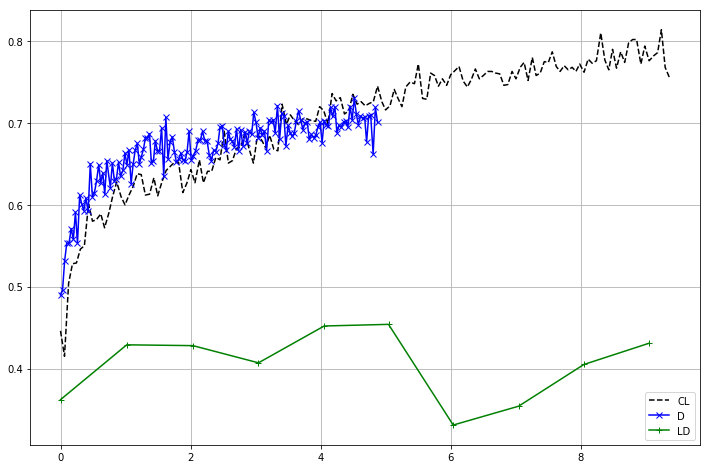
\includegraphics[width=0.65\textwidth]{content/random-block.png}
\caption{\label{fig:randomblock}Experiments with random blocks}%
\end{figure}
\todo[inline]{legenda}

